\section{Tracking the Optimized Path}

The path that will be tracked is the path that was optimized in section \ref{subsec:long_paths}. The optimized paths for both the curved and the piecewise linear path will be tracked. In addition the ground path that is to be observed will be tracked for comparison.


\subsection{Linear Path}

The result of tracking the linear ground path and the optimized path can be seen in Figure \ref{fig:lin_sim_res}. It is clear that when tracking the ground path the biggest problem is that the path that is being tracked consists of linear corners, causing abrupt changes in the roll angle of the aircraft. When tracking the optimized path on the other hand, the are no abrupt changes in the roll angle. The smooth reference path gives a smooth flight path, and the camera centre point stays focused on the ground path without any major deviations.

When comparing the attitude of the two simulations, it is clear that the optimized path gives a much more stable flight. Not only do the roll angle vary less, the pitch angle is also close to zero throughout the flight. When tracking the ground path the pitch has some variations, that will further add to movement in the camera position. 

\begin{figure}
	\makebox[\textwidth][c]{
	\subfloat[UAV position when tracking ground path]{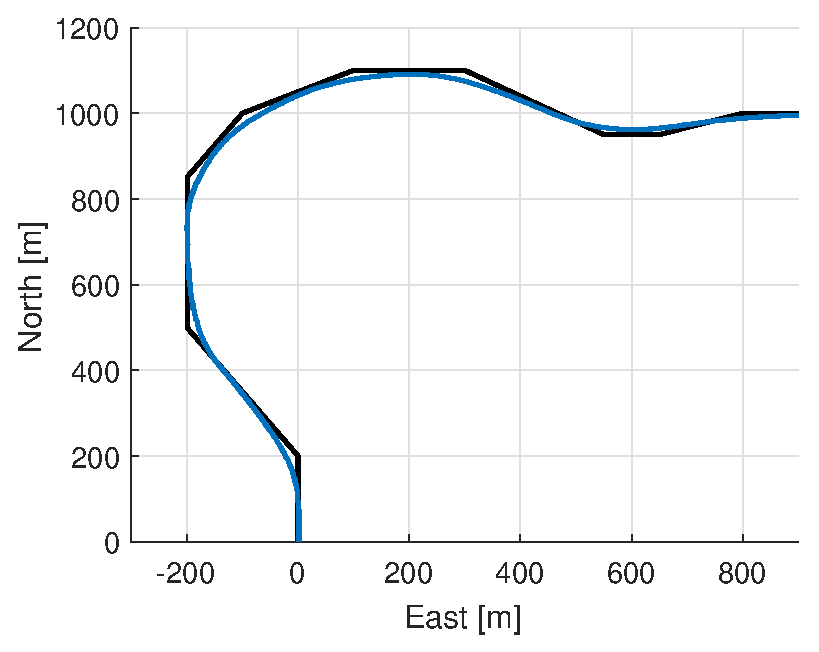
\includegraphics[width=0.5\textwidth, keepaspectratio=true]{../../results/sim/easy_path/fig_lin/path_run_UAV.eps}}
	\qquad
	\subfloat[UAV position when tracking optimal path]{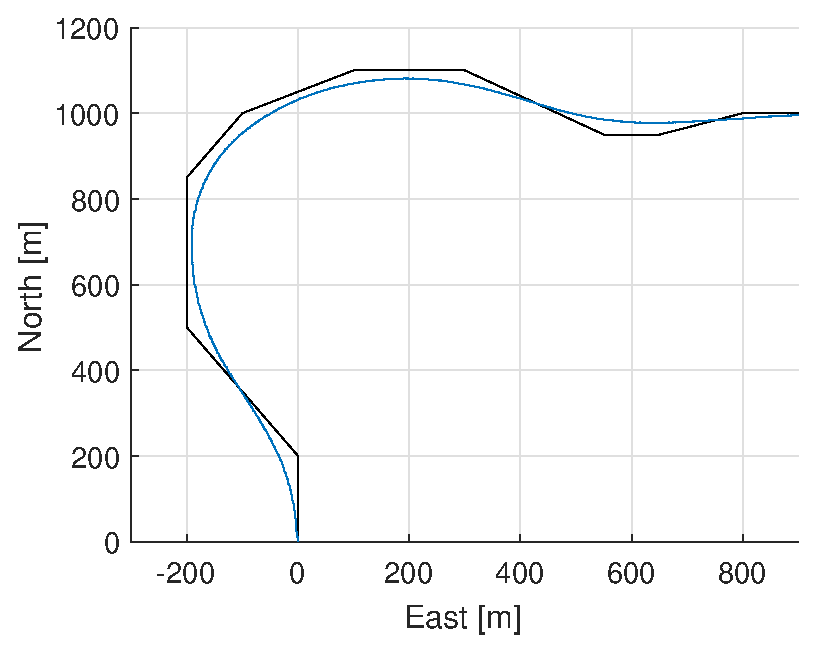
\includegraphics[width=0.5\textwidth, keepaspectratio=true]{../../results/sim/easy_path/fig_lin/pos_run_UAV.eps}}}
    
    \makebox[\textwidth][c]{
	\subfloat[Camera position when tracking ground path]{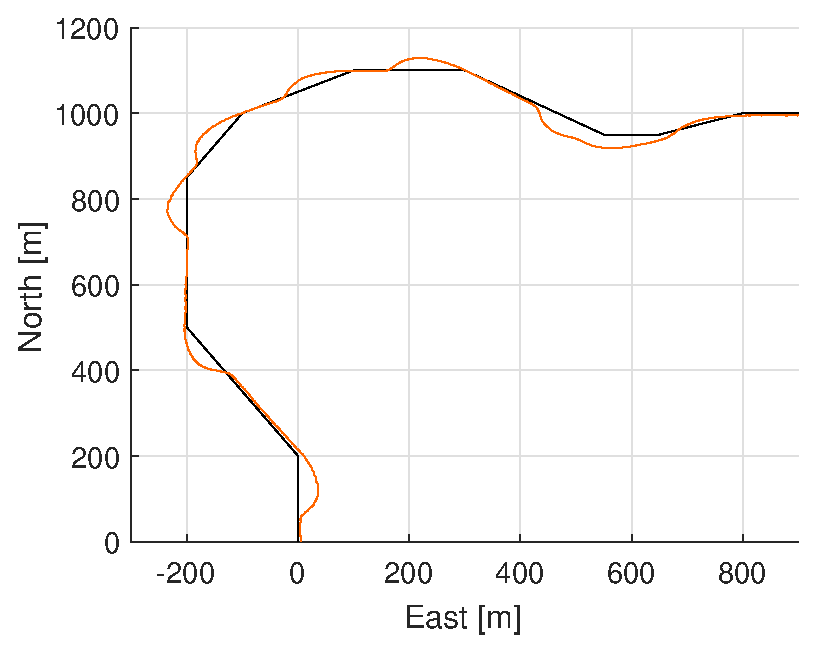
\includegraphics[width=0.5\textwidth, keepaspectratio=true]{../../results/sim/easy_path/fig_lin/path_run_cam.eps}}
	\qquad
	\subfloat[Camera position when tracking optimal path]{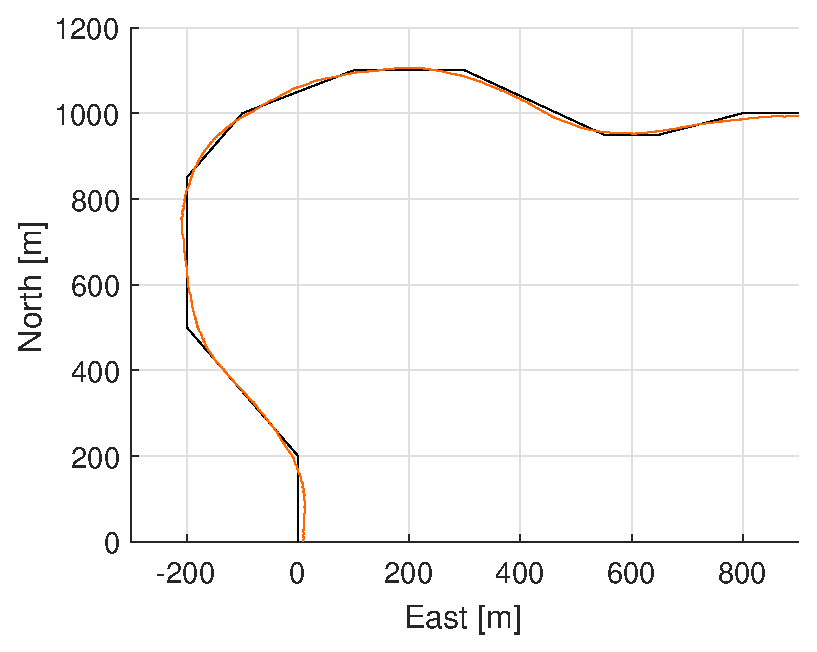
\includegraphics[width=0.5\textwidth, keepaspectratio=true]{../../results/sim/easy_path/fig_lin/pos_run_cam.eps}}}
    
    \makebox[\textwidth][c]{
	\subfloat[Attitude angles when tracking ground path]{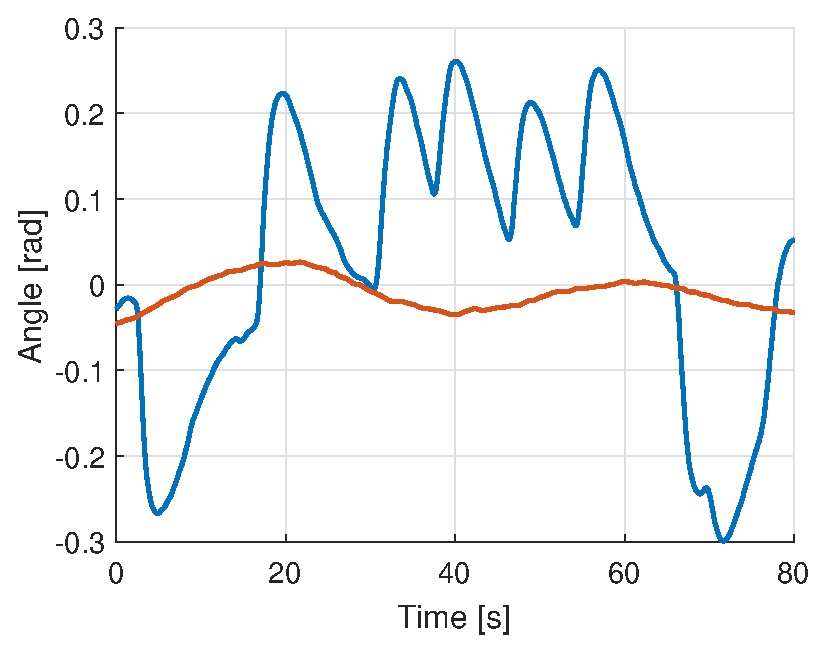
\includegraphics[width=0.5\textwidth, keepaspectratio=true]{../../results/sim/easy_path/fig_lin/path_run_attitude.eps}}
	\qquad
	\subfloat[Attitude angles when tracking optimal path]{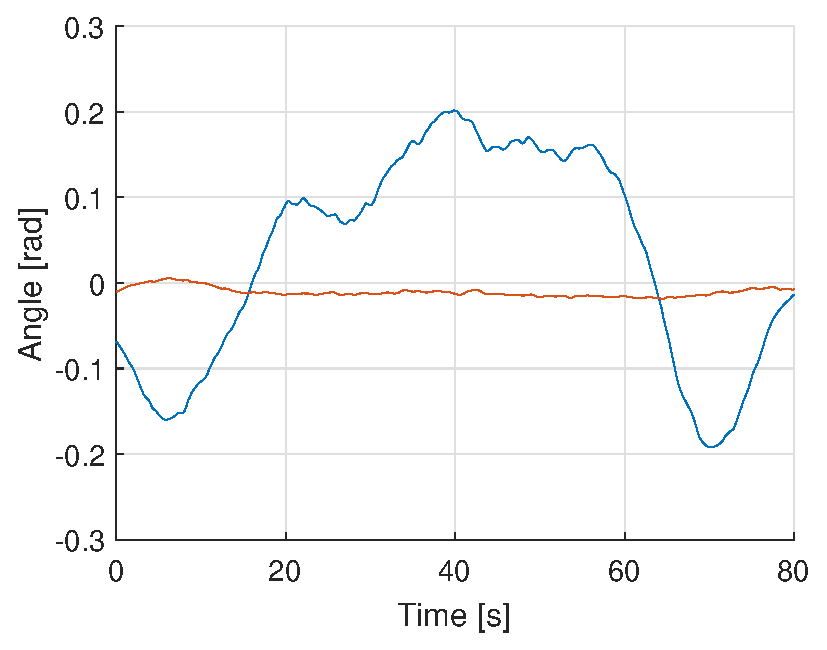
\includegraphics[width=0.5\textwidth, keepaspectratio=true]{../../results/sim/easy_path/fig_lin/pos_run_attitude.eps}}}
	\caption{The result when tracking the ground path and the optimized path.}
	\label{fig:lin_sim_res}
\end{figure}



\subsection{Curved Path}

The results for tracking the optimized curved path is very similar to the results for the optimized linear tracking. The biggest difference is that when tracking the curved ground path, the oscillations are smaller than for the linear ground path. The oscillations for the curved optimized path are also slightly smaller than for the optimized linear path, but this difference is so small that it has no practical significance.

\begin{figure}
	\makebox[\textwidth][c]{
	\subfloat[UAV position when tracking ground path]{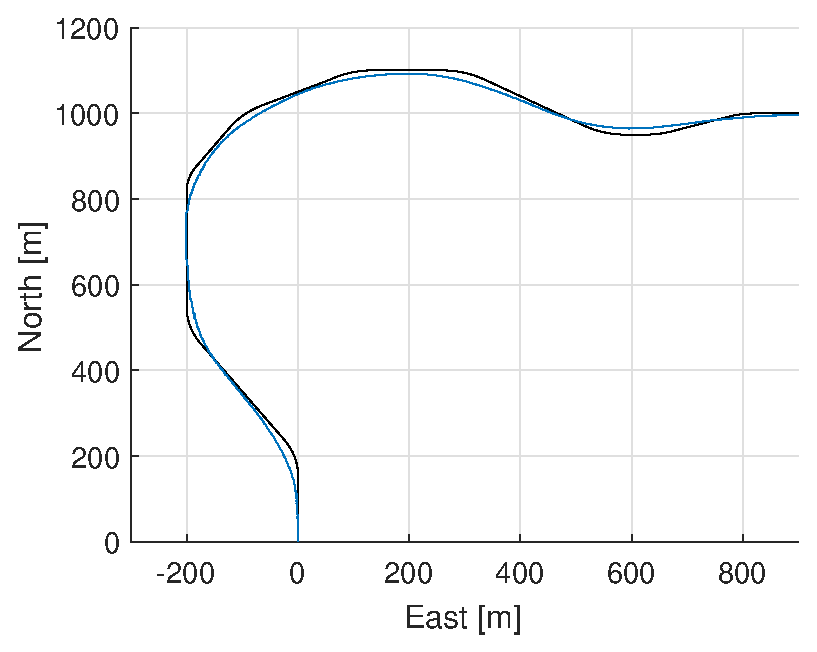
\includegraphics[width=0.5\textwidth, keepaspectratio=true]{../../results/sim/easy_path/fig_cur/path_run_UAV.eps}}
	\qquad
	\subfloat[UAV position when tracking optimal path]{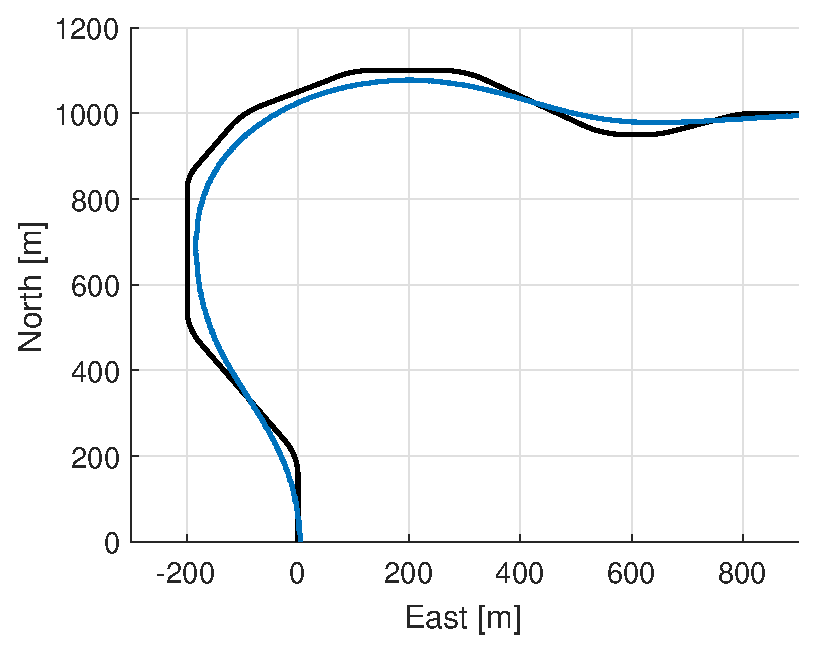
\includegraphics[width=0.5\textwidth, keepaspectratio=true]{../../results/sim/easy_path/fig_cur/pos_run_UAV.eps}}}
    
    \makebox[\textwidth][c]{
	\subfloat[Camera position when tracking ground path]{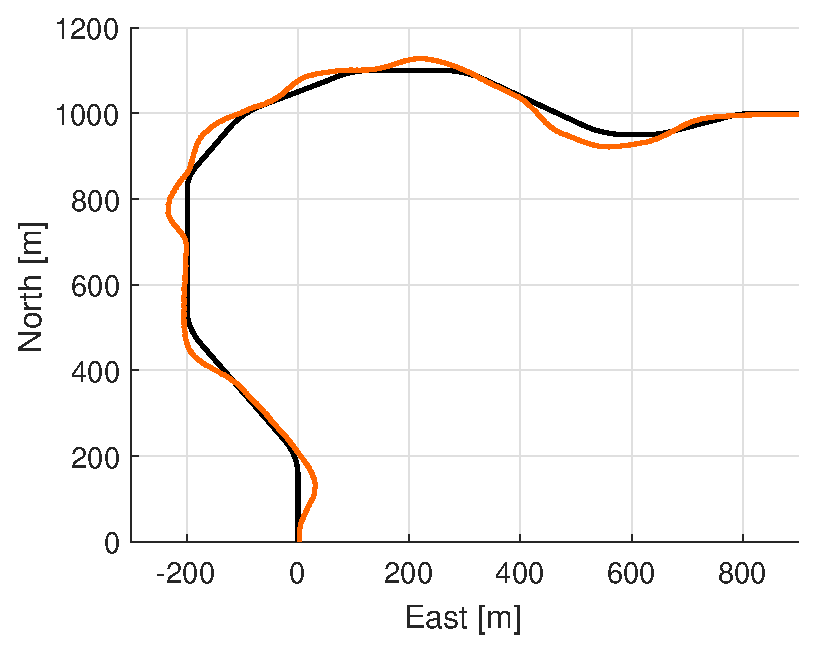
\includegraphics[width=0.5\textwidth, keepaspectratio=true]{../../results/sim/easy_path/fig_cur/path_run_cam.eps}}
	\qquad
	\subfloat[Camera position when tracking optimal path]{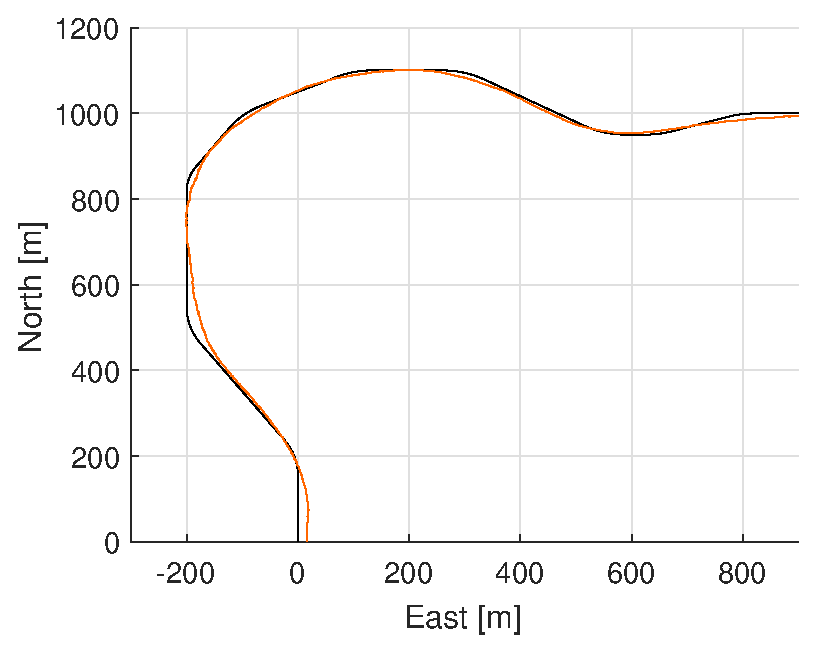
\includegraphics[width=0.5\textwidth, keepaspectratio=true]{../../results/sim/easy_path/fig_cur/pos_run_cam.eps}}}
    
    \makebox[\textwidth][c]{
	\subfloat[Attitude angles when tracking ground path]{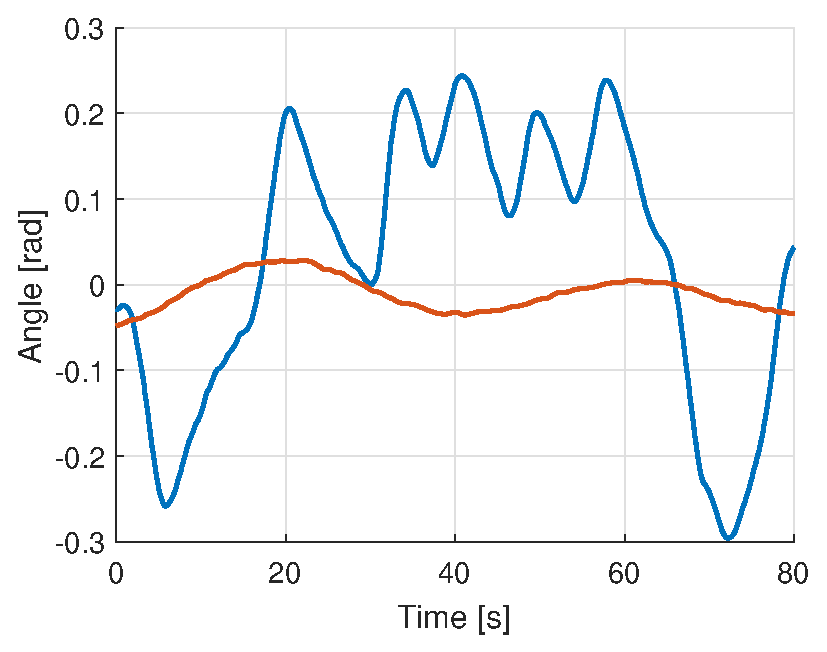
\includegraphics[width=0.5\textwidth, keepaspectratio=true]{../../results/sim/easy_path/fig_cur/path_run_attitude.eps}}
	\qquad
	\subfloat[Attitude angles when tracking optimal path]{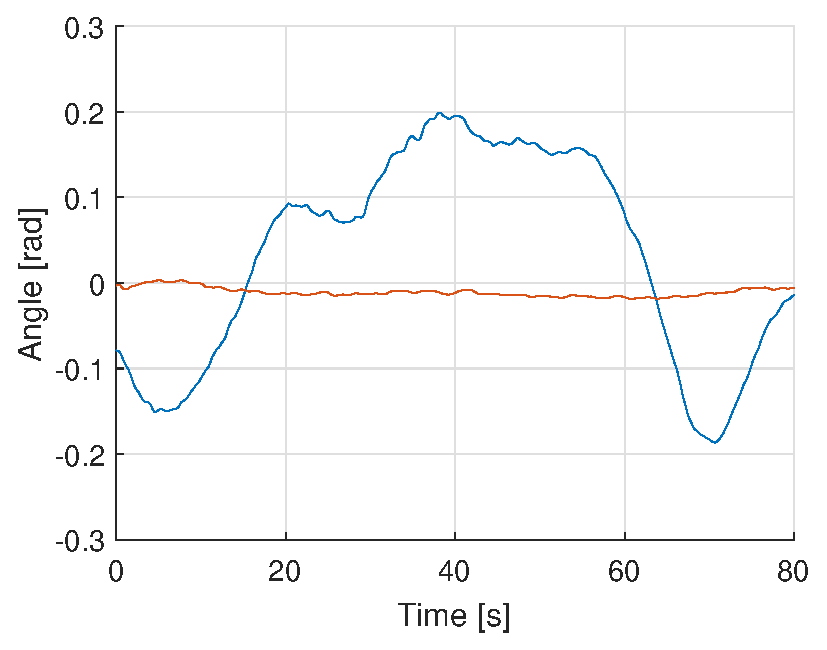
\includegraphics[width=0.5\textwidth, keepaspectratio=true]{../../results/sim/easy_path/fig_cur/pos_run_attitude.eps}}}
	\caption{The result when tracking the ground path and the optimized path.}
	\label{fig:cur_sim_res}
\end{figure}



\subsection{Linear VS. Curved}

\begin{table}[h]
\centering
\begin{tabular}{l c c c}
    \hline
    & Mean & Max  & STD \\
    \hline
    Optimized Curved Path & 4.0366m & 21.6539m & 5.0647m  \\
    Optimized Linear Path & 3.5139m & 18.4791m & 4.0691m  \\
    Ground Curved Path    & 8.0423m & 36.4857m & 10.4101m \\
    Ground Linear Path    & 7.9658m & 40.5172m & 11.2268m \\
    \hline
\end{tabular}
\caption{Mean error, max error and the standard deviation between camera centre point and ground path when tracking the path.}
\label{tab:sim_easy}
\end{table}

The statistics for the simulations of the paths can be seen in Table \ref{tab:sim_easy}, and they show that the performance when tracking the optimized linear path is better than when tracking the optimized curved path. The mean deviance is $0.5$m smaller for the linear path than for the curved path, and the maximum deviance when tracking the linear path is a little more than $3$m better than for the curved path. This is opposite of the results when optimizing the paths, where the curved path had a better tracking. It is also worth noting that mean error when optimizing the paths was bigger than the mean error when simulating the paths, and tracking the optimized paths give a considerably better result than tracking the ground path.


\subsection{Camera Field of View}

In Figure \ref{fig:fov} the field of view has been added to the camera footpring, in order to show what would be captured by an actual camera. The field of view is set to $19\degree$, which is approximately the same as the camera used in \cite{hymsySUOMALAINEN}. The figure shows that either if the ground path is tracked or the optimized path is tracked, the ground path that is to observed will be within the camera footprint. In other words, the path simulated here is a bit to simple to really show the benefits of using the optimized paths. However, it is still clearly visible that the optimized path results in a much more stable image.

\begin{figure}
	\makebox[\textwidth][c]{
	\subfloat[Ground Path]{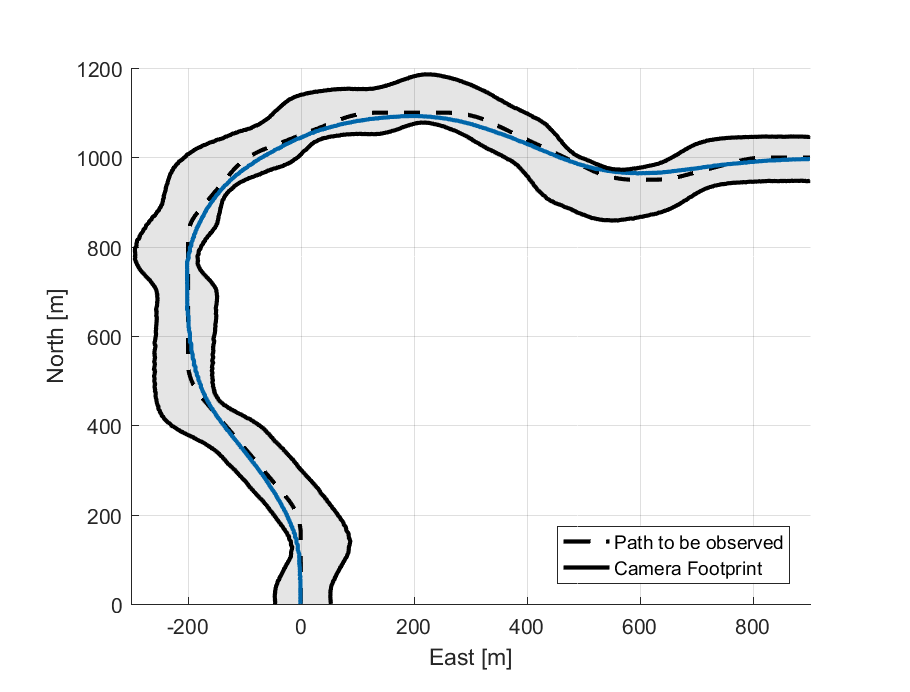
\includegraphics[width=0.8\textwidth, keepaspectratio=true]{../../results/sim/easy_path/fig_cur/path_run_fov.eps}}}
	\makebox[\textwidth][c]{
	\subfloat[Optimized Path]{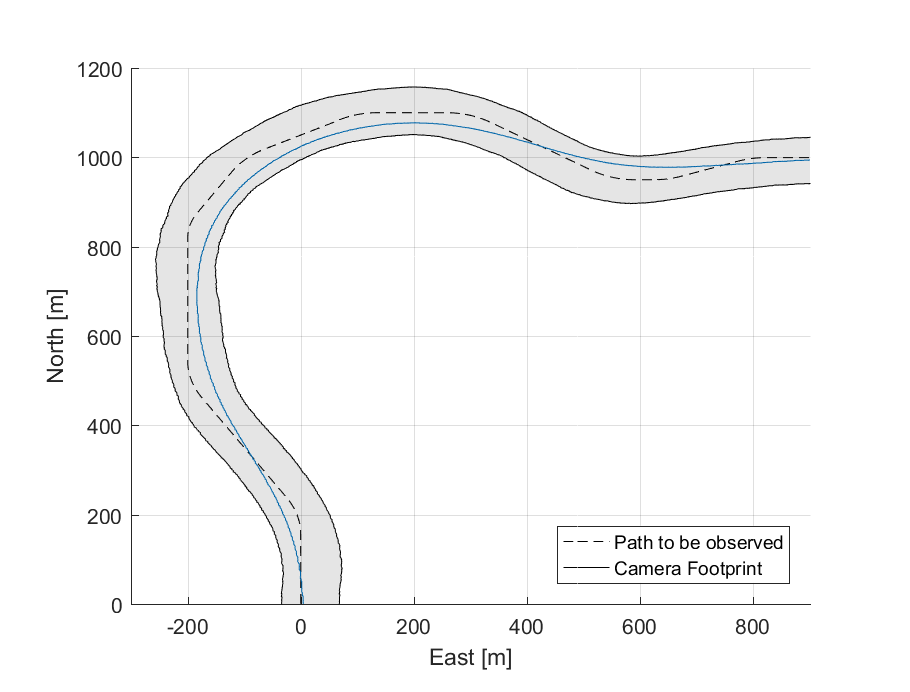
\includegraphics[width=0.8\textwidth, keepaspectratio=true]{../../results/sim/easy_path/fig_cur/pos_run_fov.eps}}}
	\caption{The field of view of the camera.}
	\label{fig:fov}
\end{figure}
